\documentclass[conference]{IEEEtran}
\usepackage[utf8]{inputenc}
\usepackage{cite}

\ifCLASSINFOpdf
  \usepackage[pdftex]{graphicx}
  \graphicspath{{.}{images/}{pdf/}{jpeg/}}
  \DeclareGraphicsExtensions{.pdf,.jpeg,.png}
\else
  \usepackage[dvips]{graphicx}
  \graphicspath{{.}{images/}{../eps/}}
  \DeclareGraphicsExtensions{.eps}
\fi

\usepackage[caption=false,font=footnotesize]{subfig}

\usepackage{url}
\usepackage{hyperref}
\hypersetup{ 
colorlinks,% 
citecolor=black,% 
filecolor=black,% 
linkcolor=black,% 
urlcolor=Blue 
}
\usepackage[usenames,dvipsnames]{xcolor}

% correct bad hyphenation here
\hyphenation{op-tical net-works semi-conduc-tor}

\renewcommand{\baselinestretch}{0.952}
\begin{document}

\title{Community-Lab: vision and architecture of a community networking testbed for the Future Internet}


% author names and affiliations
% use a multiple column layout for up to three different
% affiliations
%\author{%
%\IEEEauthorblockN{Xavier León, Felix freitag, Leandro Navarro\\and Ester López}
%\IEEEauthorblockA{%
%Universitat Politècnica de Catalunya\\
%Barcelona, Spain\\
%\texttt{\{xleon, felix, leandro, esterl\}@ac.upc.edu}}
%\and
%\IEEEauthorblockN{Axel Neumann and Ivan Vilata}
%\IEEEauthorblockA{Pangea.org\\
%NGO Internet Solidario\\
%Barcelona, Spain\\
%\texttt{neumann@cgws.de, ivan@pangea.org}}
%\IEEEauthorblockN{Pau Escrich and Roger Baig}
%\IEEEauthorblockA{guifi.net\\
%Community Network\\
%Catalonia, Spain\\
%\texttt{\{pau, roger\}@guifi.net}}
%}

\author{%
\IEEEauthorblockN{%
Axel Neumann\IEEEauthorrefmark{1},
Ivan Vilata\IEEEauthorrefmark{1},
Xavier León\IEEEauthorrefmark{2},
Pau Escrich\IEEEauthorrefmark{3},
Leandro Navarro\IEEEauthorrefmark{2},
Ester López\IEEEauthorrefmark{2}%
}
\IEEEauthorblockA{%
\IEEEauthorrefmark{1}Pangea.org NGO, Barcelona, Spain\\
\texttt{neumann@cgws.de, ivan@pangea.org}}
\IEEEauthorblockA{%
\IEEEauthorrefmark{2}Universitat Politècnica de Catalunya, Barcelona, Spain\\
\texttt{\{xleon, leandro, esterl\}@ac.upc.edu}}
\IEEEauthorblockA{%
\IEEEauthorrefmark{3}guifi.net Community Network, Catalonia, Spain\\
\texttt{pau@guifi.net}}
}

\maketitle


\begin{abstract}
Community networks are an emerging and successful model for the Future Internet
across Europe and far beyond. The CONFINE project complements existing FIRE (Future Internet
Research and Experimentation) infrastructures by establishing Community-Lab,
a new facility built on the federation of existing community IP networks constituted by more than 20,000 nodes and 20,000 Km of links. These unique infrastructures pose an interesting set of challenges different from existing testbeds. In this paper we present the benefits of having such testbed for the research community as well as the improvement and evolution of community networks themselves. Additionally, we sumarize the challenges encountered and describe our long-term vision for the community network testbed and its current state of implementation.
\end{abstract}

\section{Introduction}

In the recent years, the perception of the key role of Internet access for the
digital society and the size, growth and scope of the Internet has put under stress
its architecture and protocols. The growing Internet penetration at homes, schools,
workplaces, and any public or private organization, and the introduction of very demanding
and QoS-sensitive applications like distribution of large files, interactive multimedia,
real-time audio and video result in an explosive growth in the demand for capacity.

However, the characteristics of the investment needs, cost of ownership, and expected return
of investments outside the traditional telecommunication markets in rural areas or in 
urban areas with low income individuals or special needs not covered by standard products
make those areas very unattractive for traditional telecom providers. It has lead to the
appropriation of these strategic technologies by the communities themselves, by means of
self-provision, self-ownership and self-operation. These underserved areas have taken their
connectivity needs into their own hands, hence, they developed into ``community networks''.

Community networking (also known as bottom-up networking) is an emerging model 
for the Future Internet across Europe and beyond where communities
of citizens build, operate and own open IP-based networks, a key infrastructure
for individual and collective digital participation.

These ``community networks'' (CN) are part of the Internet but differ in several key
aspects due to their nature: they are open and transparent as there are no barriers of entry
for participation; governance and knowledge is open, with public documentation on
every technical and non-technical aspect; they are self-owned as community members
own the network; self-managed with distributed and uncoupled structure that can be open
for the participation of community members; self-growing in topology and capacity, based not only
on planning but also on immediate demand, as community members can learn and decide to extend the nework
to reach a new member or provide more capacity. Thus, these networks are not just
a path to reach the outside Internet but a local network with internal servers, services and
internal traffic connected to the Internet.

Community-Lab is a testbed being deployed by the CONFINE European
Integrated Project\footnote{\url{http://www.confine-project.eu}}. This testbed supports experimentally-driven research
on community-owned open local IP networks. It integrates and extends 
three existing community networks: Guifi.net (Catalonia, Spain),
FunkFeuer (Wien, Austria) and AWMN (Athens, Greece); each is in the
range of 500 -- 20,000 nodes, a greater number of links and even more end-users.
These networks are extremely dynamic and diverse. They combine
successfully different wireless and wired (optical) link technologies, static, dynamic
and ad-hoc routing schemes, and management schemes. They run multiple
self-provisioned, experimental and commercial services and applications.
This testbed provides researchers with access to these emerging
community networks, supporting any stakeholder interested in developing
and testing experimental systems and technologies for these open
and interoperable network infrastructures.

%1.1 why is research in CN important (Confine-Brochure in www.confine-project.eu)
%  - to support growth of CNs (scalability, sustainability)
%  - future internet and digital agenda

The ultimate motivation behind the deployment of such infrastructure is 
to support the growth of community networks in terms of their scalability and
sustainability by providing the means to conduct experimentally driven research. 
We expect that this research will directly impact the quality of community networks
by improving current short-commings and providing the basis for a sustainable
model of community networking.

%1.2 what research in CN (CN shortomings)
%  - howto impove privacy
%  - networking robustness (eg routing optimization, cross-layer optimizations)
%  - efficient content distribution
%  - network policies evaluation/optimization
%  - heterogenous physical networks (wireless, broadband fiber)
%  - node robustness (eg automatic reconfiguration, deployment, failure handling...)

Currently, there are several challenges and lines of research to enhance existing
community networks. Among others, CNs must consider carefully the impact on the privacy of their
users given their openness and degree of decentralization; content distribution 
should be efficient given the constrained resources by improving network robustness 
-- e.g. routing and cross-layer protocol optimizations; a critical issue is the
robustness of the nodes participating on the network (e.g. automatic reconfiguration,
deployment and failure handling, etc.) because they may sit on remote locations not
easily accessible on a day-to-day basis by community owners; and finally, CNs must handle a whole range
of heterogeneous physical networks ranging from wireless links to broadband fiber.

%1.3 why difficult to do reasearch? (Researcher shortcomings)
%   - there are no real-life CN testbeds (only small lab deployments)
%   - no existing implementations available
%   - community driven effort (not a controlled lab)

However, these challenges are being addressed currently by means of simulations 
or on very small controlled lab environments because there exists no real testbed
to experiment on, which makes the results hard to translate to real scenarios. The Community-Lab testbed
being deployed by CONFINE tries to provide such infrastructure for researchers to evaluate
their proposal on an environment with the characteristics (for the best and for the worst)
of real community networks.

\section{Related Work and Background}
\label{sec:related-work}
%= Other testbeds, what they offer (PlanetLab (Xavi knows well), and wireless
%testbeds that are known from papers (Berlin testbeds, Nitos, ...?)

There are several initiatives in Europe without considering the three CNs participating in this initial
phase of the testbed --guifi.net (Catalonia, Spain), FunkFeuer (Wien, Austria) and AWMN (Athens, Greece). The Berlin RoofNet project is an
experimental mesh network in Berlin consisting of nearly 50 indoor nodes mainly to provide
students with Internet access as well as VoIP \cite{berlin-roofnet}. In the USA there are similar initiatives as well. Cities like New York, Seattle, Washington or Austin cooperate with
public and non-profit organizations to develop and improve free wireless hotspots within 
their cities to provide citizens with Internet access. Also, the MIT Roofnet \cite{mit-roofnet} project
is a mesh network consisting of about 50 nodes and covers an area of about four square
kilometers allowing for small scale and controlled experimentation thanks to the
Click Modular router integrated within their firmware. 

However, all these wireless network deployments 
are expected to provide a service (Internet connectivity mainly) to users and do not
cover the necessity of researchers to perform experimentation on top of them.

% Ivan: I need a small introduction to the concept of slice and sliver.

The first initiative of a large-scale testbed to conduct experimental research was introduced by PlanetLab \cite{planetlab}.
They currently manage a planetary-scale experimental testbed composed of hundreds of nodes to deploy and
evaluate distributed applications and services in a real environment. The key characteristic of this
testbed is the concept of resource sharing (given their scarcity) among different researchers by means of
virtualization. PlanetLab introduced a basic abstraction called \textit{slice} which enables the isolation
of different experiments. A \textit{slice} is an orthogonal fraction 
of the testbed, or in other words, a set of nodes on which applications are assigned a fraction of resources by means of a
kind of virtual machine called \textit{sliver}. This concept of \textit{slice} has evolved over time to also
account for network isolation and other types of resources.

If we look at the wireless research area, there are also several initiatives to create a testbed to conduct
experimental research, but none of them address the problem of high scale deployments nor sharing of resources -- two
of the main principles behind Community-Lab. For instance, the IBBT w-iLab \cite{ibbt} in Flanders (Belgium), 
consists of mainly 200 indoor locations spread across three office floors and is mainly composed of sensor networks. In
Greece, the NITOS \cite{nitos} testbed enables researchers to completely control the software on the testbed nodes, which denies 
the possibility of several simultaneous users. Besides, it consists of 40 WiFi nodes which only enables 
small scale experiments. Finally, the ORBIT testbed \cite{orbit} is a large
indoor two-dimensional grid of around 400 802.11 radio nodes which can be dynamically interconnected
into specified topologies, which makes it the largest indoor wireless lab.


\section{Challenges and Requirements}

% Ivan: I need a reference to slice and network isolation.

% 2. what challenges it poses to develop a testbed on top of it. ( 1 page )
%  - keep stability and security
%  - keep CN privacy / Network Isolation
%  - researcher affiliation != testbed management ?!= node ownership
%  - usablitiy (simple API despite system complexity)
%  - not CPU powerful devices (cheap)
%  - remote locations
%  - connection instability, variable connectivity and available bandwidth
%  - cross-CN communication (testbed spanning several CNs)
%  - lack of IPv6 support in existing CNs (tinc workaround)
%  - Development and Debugging facilities (VCT)

Deploying, managing, and using experimentation facilities in an
existing CN, where ownership and administration of network
infrastructure is divided over many entities, imposes a set of new
challenges and requirements to the design of the Community-Lab
architecture. A selection of most important requirements is briefly
discussed by the following subsections.


\subsection{Lightweight, Low Cost, Free, and Open Source}
% Lightweight, Low Cost, Free, and Open Source approaches are important
% to keep equippment and maintainace cost low, ease reviewing and
% contribution efforts, and to aim for sustainability and acceptance in
% the free networks communities.

In order to achieve a widespread deployment of CN nodes supporting the
Community-Lab testbed, existing installations must be extended with new
components which comes with additional equipment acquisition and
maintenance cost (e.g. increased energy consumption) for the node
owners. Therefore, lightweight and low cost solutions are important to
keep expenses as low as possible.

Reusing of generally accepted approaches and free and open source
software is mandatory to ease reviewing and trust, lower the burden
for contribution, and to aim for sustainability and acceptance in the
free networks communities.

\subsection{System Stability}

To facilitate the preparation and execution of experiments,
researchers should be provided with an environment they are familiar
with and which allows them to reuse already existing implementations
and prototypes.  Such environment is given by a Linux OS in
combination with root permissions which has evolved to a de-facto
standard environment for networking experiments.

On the other hand, from a security point of view, it must be ensured
that experiments enabled with root permissions can not affect the
general Community-Lab Node System. This can be achieved by isolating
experiments on dedicated hardware or with virtualization techniques.
But, despite many mature virtualization solutions exist for UNIX
systems, few of them have been successfully ported to embedded
hardware which is commonly used for nodes in CNs.

\subsection{Network Stability}
%Stability of production network must be ensured despite potentially
%harmfull experiments.
Since the Community-Lab testbed aims to enable community integrated network
experiments, some (controlled) level of interaction between the
experiments and the main CN must be possible. On the other hand it
must be ensured that experiments do not interfere seriously with each
other nor with the production network.  The potential harm of
experiments can be classified into two types:

\begin{itemize}

\item Resource Consumption: It must be ensured that each experiment
  gets a limited but fair share of the available link capacities.
  Traffic Shaping and Distributed Rate Limiting techniques can be used
  here.

\item Conflicting Protocol Behavior: Experimentation with key network
  services (medium access control, routing, DNS) and other protocol
  resources (address, port, channel assignments) must be isolated or
  rigorously controlled.  Firewall or Software Defined Networking
  techniques (like VLAN tagging) or even the complete physical
  isolation of link resources are considered depending on the lowest
  accessed network layer of the experiments.

\end{itemize}

\subsection{Privacy of CN users}
%Privacy of CN users must be ensured while enabling researchers to do
%measurements and observations.

While researchers should be conceptually enabled to collect user
and network data (for statistical evaluation or as real-time feedback
for protocols), privacy regulations of the corresponding CN licences
and peering agreements must be respected.
Therefore, the CONFINE system must provide convenient mechanisms for
traffic filtering and anonymization of networking data before it is
provided to researchers.

\subsection{Management Robustness}
%Management system should be robust against potential connection
%instabilities to remote experimentation facilities.

One of the interesting characteristics for research in real-life CNs
is the variety of link setups and stabilities that arise due to the
distributed management of CN infrastructure and the objective to provide
connectivity even to remote locations at low cost. Often, such
locations are abandoned by commercial ISPs because of deployment
challenges and poor revenue perspectives.

Therefore, the system (in charge of managing the distributed
experiments in Community-Lab enabled nodes) must be prepared to deal with
connectivity starvation and the spontaneous appearance and outage of
links and nodes.


\subsection{IP-Address Provisioning}
%IP address provisioning for experiments despite common scarcity of
%IPv4 address space and incomplete IPv6 support in many CNs

The objective to allow active experiments on top of existing CN
infrastructure as well as interaction with users demands the
provisioning of CN public IP addresses for slivers.

However, due to the general scarcity of IPv4 address space, the
allocation of unique addresses for experiments is difficult. Also,
many CNs are using their own address allocation schemes based on the
limited private address ranges for internal routing and end users.

This non-coordinated allocation of IPv4 addresses is raising another
challenge for the long-term objective to enable federation of Community-Lab
testbeds deployed in different CNs.

Relying on IPv6 seems the natural solution to this challenge but we must
consider the fact that only few existing CNs yet support native IPv6
routing.

\subsection{Compatibility}
%Compatibility to variety of existing CN models and heterogeneity of
%used (often proprietary) soft- and hardware solutions.

Apart from the general requirement for the Community-Lab architecture to be
compatible with the different networking models employed by CNs, the
Community-Lab Node System must be compatible with the original system used on
nodes in the CN.

Because nodes in CNs are setup individually and may be based on
proprietary and closed software systems, no modifications to the
original community node firmware should be required and only few
assumptions should be made on supported features or the concrete
implementation of a node.


\subsection{Role-specific APIs and Usability}
%Role-specific APIs and access control should be provided for testbed
%management, node owners, and researchers.
%Usability -- Tools and APIs for managing and deploying a CONFINE
%testbed should be as simple and intuitive as possible (for each
%involved role and despite the intrinsic complexity).

The operation, deployment and usage of a testbed integrated in
existing CNs involves different roles. In particular, the roles of
testbed managers, node owners, and researchers have been identified.

In order to simplify the operations related to each role and prevent
misconfigurations due to overlapping or missing responsibilities,
role-specific APIs  and access control should be provided.

Finally, the tools and APIs provided for managing and deploying a
CONFINE testbed should be as simple and intuitive as possible (for
each involved role and despite the intrinsic complexity).



%\subsection{Development Environment}
%A Development environment is needed, allowing testing and
%debugging of new software components before being installed into
%real-life CNs.




\section{Community-Lab testbed architecture}
\label{sec:confine-architecture}

A CONFINE testbed like Community-Lab consists of at least one \emph{server} or \emph{controller}
and a set of \emph{nodes} which can be spread over several community networks
(CNs).  A server is a normal computer which is publicly reachable inside of a
CN.  A node can be an integral part of a CN: in contrast with a boundary host,
a Community-Lab node can relay other CN traffic not related with the testbed.

The design described in this section intends to facilitate the addition of
Community-Lab nodes in any location of a CN by connecting additional devices to
existing CN ones with minimum or no testbed-specific changes to their
configuration.  At the same time, it provides researchers with familiar
Linux environments with root access and rich connectivity
options (see \ref{sec:connectivity}) including:

\begin{itemize}
\item Simple NAT access (like that of most home computers).
\item Public CN addresses (to serve incoming connections).
\item Full L2 access to VLAN-tagged networks (to implement routing
  experiments).
\item CN traffic sniffing (with anonymization).
\item Raw L1 access (under certain conditions).
\end{itemize}

\subsection{Long-term vision}

\begin{figure}[!t]
\centering
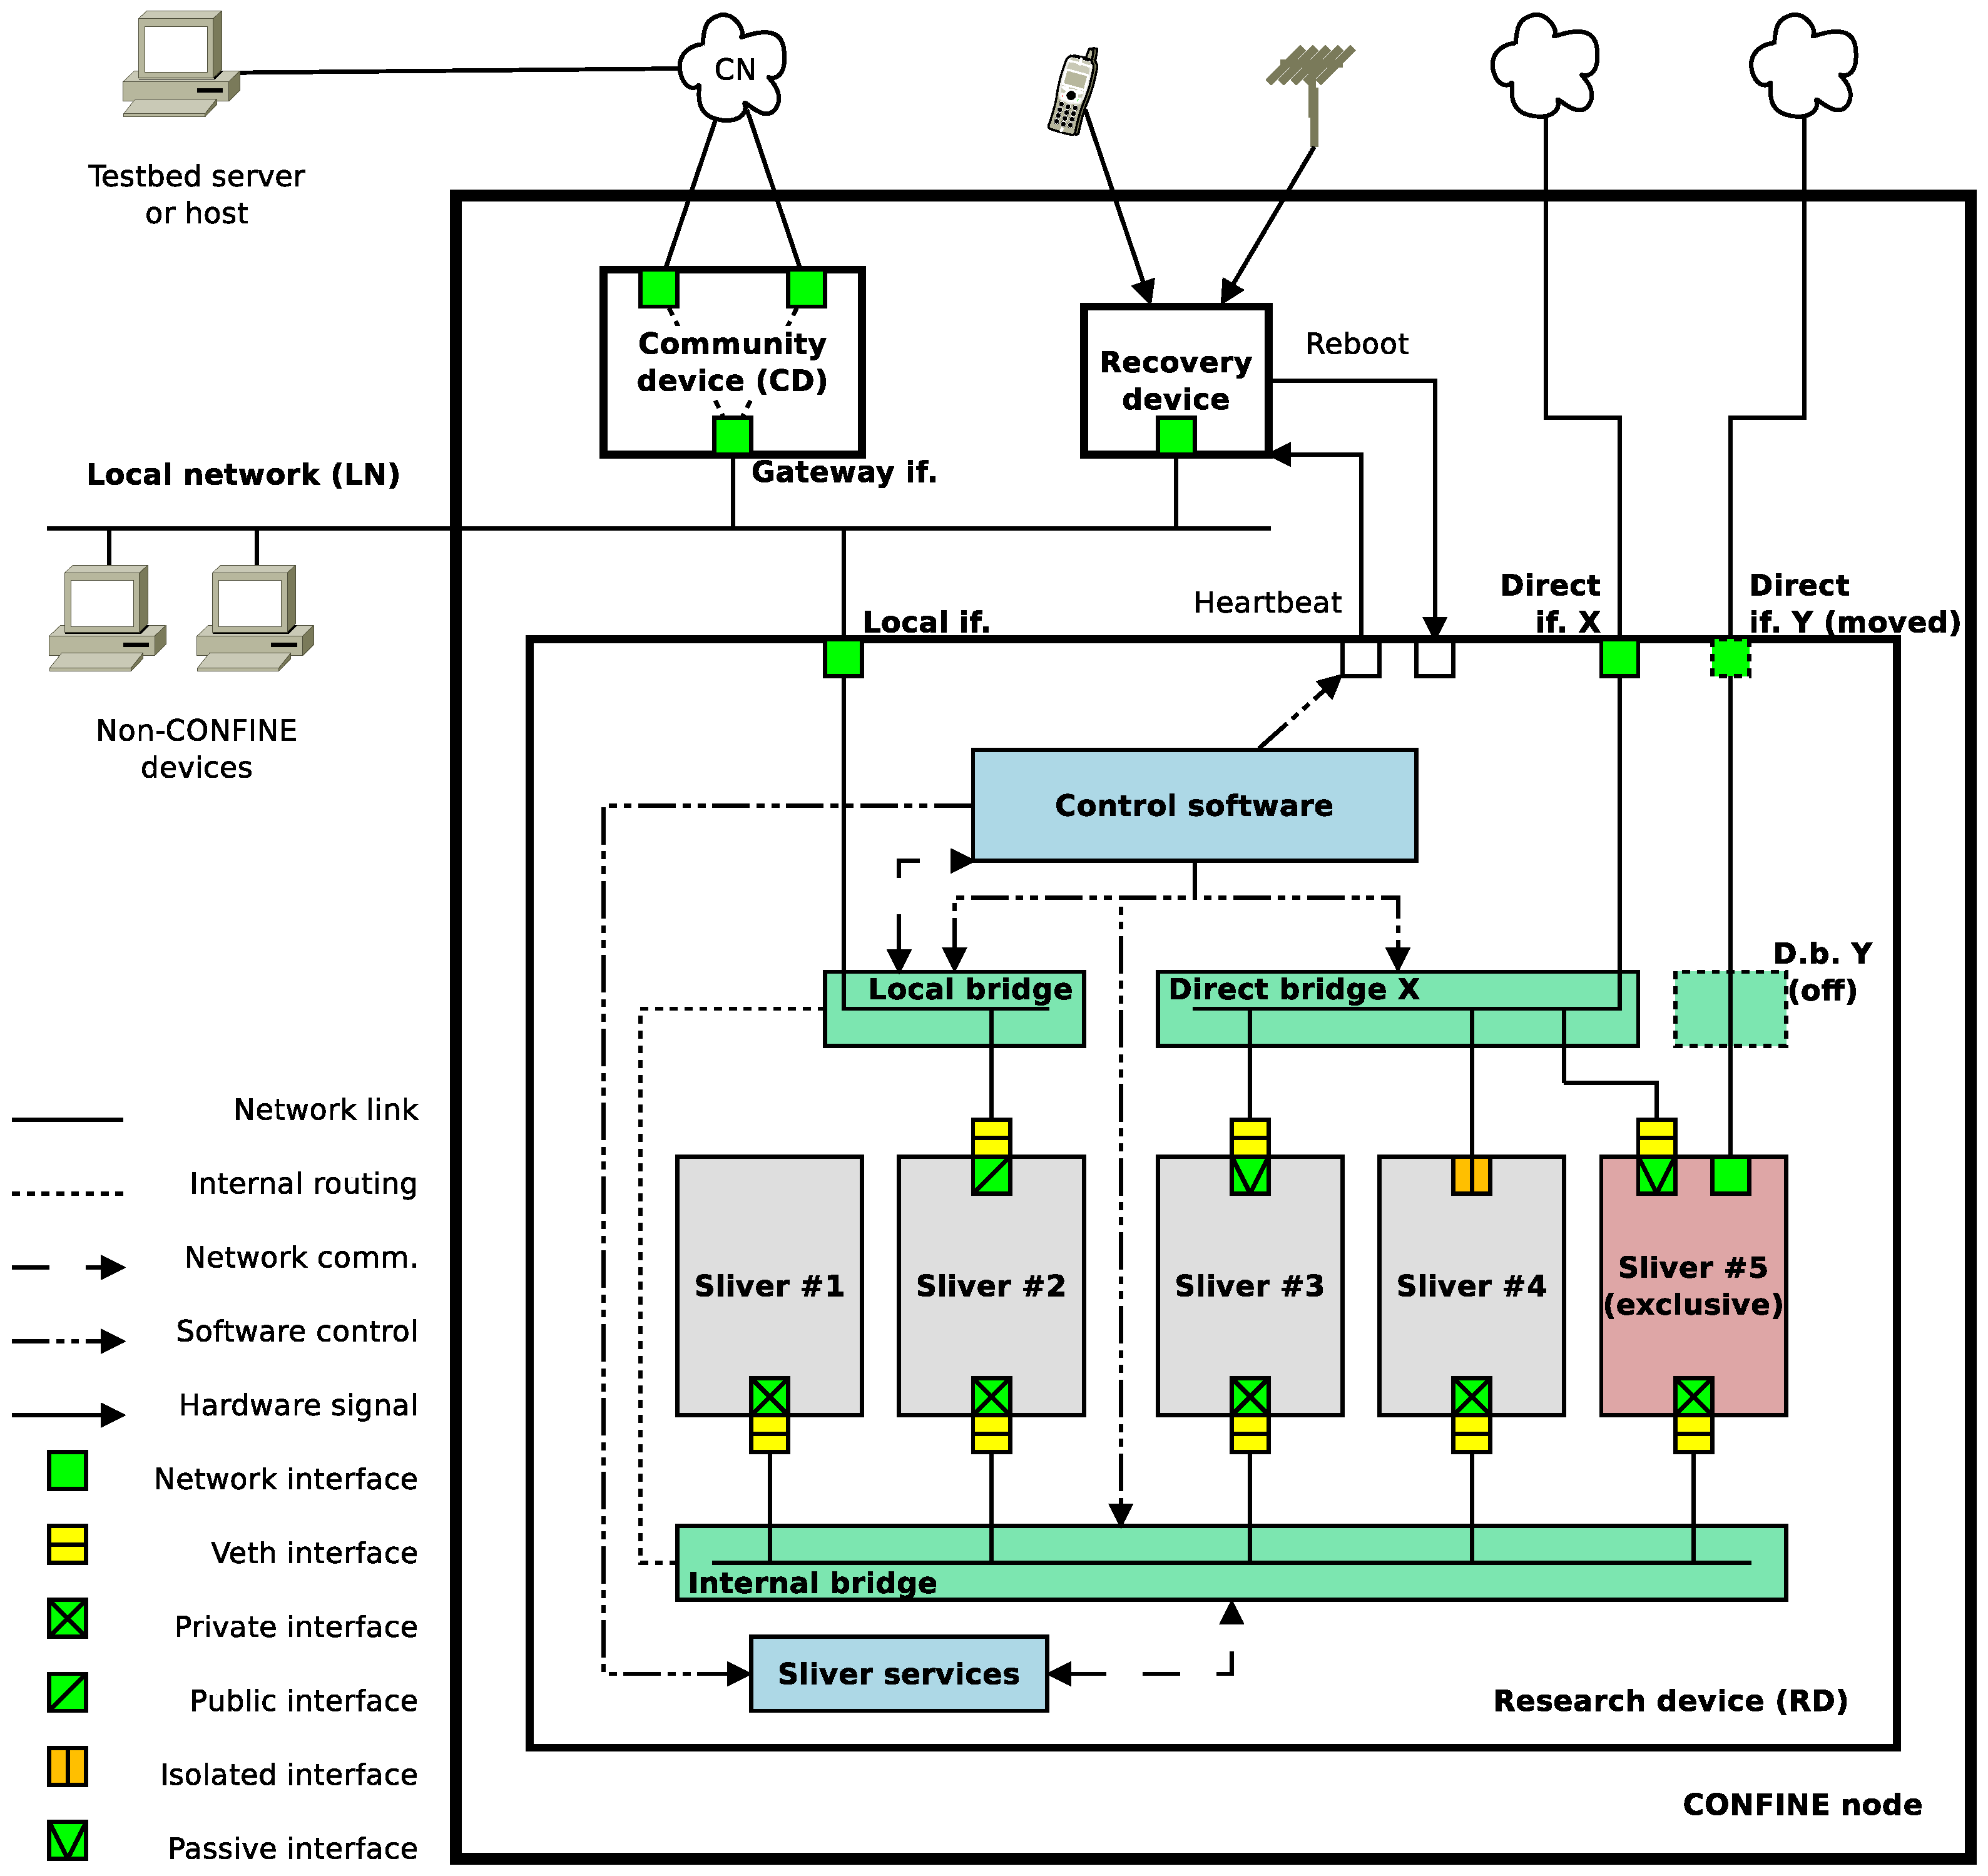
\includegraphics[width=\linewidth]{node-arch}
\caption{The architecture of a Community-Lab node.}
\label{fig:node-arch}
\end{figure}

As shown in figure \ref{fig:node-arch}, a \textbf{Community-Lab node} (node)
consists of two or three devices: the \textbf{community device} (CD), the
\textbf{research device} (RD) and an optional \textbf{recovery device}.  This
separation tries to preserve the stability of the CD (and thus of the CN) and
is most compatible with any frmware it may run.  All devices in a node are
linked by a wired \textbf{local network} (LN), possibly shared with other
non-testbed devices like CN clients using the CD as a gateway.

\subsubsection{The community device}

The CD is a \emph{completely normal community network device} with at least
two different network interfaces: a wired or wireless one connecting to the CN
(a \textbf{community interface} with a \textbf{community address}) and a wired
one to the LN (the \textbf{gateway interface} with its \textbf{gateway
  address}).  It can act as a simple gateway for hosts connected to the LN,
some of them with fixed addresses not assigned to other devices via DHCP or
similar.  This allows the use of a uniform address scheme for testbed elements
in the node.

The node is accessed by testbed servers, administrators and researchers via
the community interfaces of the CD, although node administration may
occasionally proceed directly through the LN.

\subsubsection{The research device}

The RD is a relatively powerful device (compared to the CD) running a
\emph{customised OpenWrt firmware} provided by CONFINE which allows simultaneously running
several \emph{slivers} implemented as Linux containers \cite{lxc}.
Slivers have limited access to the device's resources and to one another, thus
ensuring slice and network \emph{isolation}.  This is guaranteed by the
\textbf{control software} run in the RD through tools like \texttt{ebtables},
\texttt{arptables}, \texttt{iptables}, \texttt{tc}, Open vSwitch…

% XXXX lxc: http://lxc.sourceforge.net/ "Linux containers"

The RD implements an \textbf{internal bridge} with an \textbf{internal
  address} that is the same in all testbed nodes and which belongs to a
private network which does not clash with CN or LN addresses.  The RD offers
some basic \textbf{sliver services} (see \ref{sec:sliver-services}) on the
internal address, including NAT gateway access to the CN.

The RD also implements a \textbf{local bridge} which connects to the LN
through a wired interface (the \textbf{local interface}).  The bridge is used
for simple network layer access to the CN through the CD's gateway address,
and the \textbf{local address} of the RD in it is fixed and used for testbed
management and remote administration.  For easy RD setup and local
administration, the local interface may also sport a \textbf{recovery address}
that is easily predictable or the same in all testbed nodes and that belongs
to a private network which does not clash with CN or LN addresses (nor those
of the internal bridge).  A \textbf{debug address} which is also private and
easily predictable can be used to access different RDs in the same local
network for debugging purposes.

The RD may have additional \textbf{direct interfaces}, each one connected to
its own \textbf{direct bridge}.  These interfaces may be connected to the CN
at the link layer and used for experiments below the network level (see
\ref{sec:connectivity}).

All the aforementioned bridges are managed by the control software in order to
ensure network isolation between slices (i.e. between slivers running in the
RD) as mentioned above, and to keep CN stability and privacy.

\subsubsection{The recovery device}

The node may include some simple recovery device whose purpose is to
\emph{force reboot} of the RD in case of malfunction using some direct
hardware mechanism (like a GPIO port connected to the power supply of the RD),
thus avoiding the need for physical presence for rebooting devices in places
with difficult access.

The recovery device may get remote instructions from the CN (via the LN) or
via different sensors, preferably based on wide-range technologies suffering
from low interference and differing from those used by the CN (like ham radio
signals, GSM calls or SMS).  It may also receive a \emph{heartbeat signal}
kept by control software via some direct link like a serial line; when the
recovery device misses a number of heartbeats, it reboots the RD.

A more advanced version of this device may help the RD boot some recovery
environment (e.g. via PXE) or collaborate in some techniques for safe device
upgrade and recovery (see \cite{van12}) to allow restoring its firmware to a
known state.

% XXXX van12: https://archive.fosdem.org/2012/schedule/event/safe_upgrade_of_embedded_systems.html "Safe upgrade of embedded systems" Arnaut Vandecappelle, FOSDEM 2012

\subsubsection{Node and sliver connectivity}
\label{sec:connectivity}

The research and recovery devices have fixed addresses in the LN and they need
no routing protocol software to reach the CN: they simply use the CD's gateway
address as a default gateway.  Static configuration or DHCP suffice as long as
the addresses they get are fixed.

In contrast, the connectivity of a sliver is determined by the network
interfaces it sports, which are requested by the researcher at sliver
definition time and depend on the interfaces provided by the RD and their
features.  Default routing configuration is explicitly controlled by the
researcher to avoid traffic unexpectedly flowing through unwanted interfaces.

\begin{itemize}
\item Every sliver has a \textbf{private interface and address} whose host
  side \emph{veth} interface is placed in the internal bridge.  The address is
  automatically assigned from the RD's private network, thus allowing access
  to the RD's internal address and sliver services (see
  \ref{sec:sliver-services}).  The researcher may choose to use the latter
  address as the default gateway, in which case traffic is routed by the RD
  through the local bridge to the CD's gateway address after performing NAT.
  This allows \emph{client access to the CN} but not connections from the CN
  to the sliver (similar to a home computer behind a NAT gateway on the
  Internet) \emph{nor traffic between slivers}.  Thus the sliver is ensured
  that there will be no incoming connections on that interface, obviating the
  need for firewalls or access control.

  Sliver container 1 in figure \ref{fig:node-arch} only has a private
  interface in the internal bridge.

\item If the RD has been allocated some public addresses, the researcher may
  request a \textbf{public interface and address} whose host side \emph{veth}
  interface will be placed in the local bridge, thus allowing access to the
  LN.  The address is automatically assigned from the RD's pool of public addresses, and
  the researcher may choose to use the CD's gateway address as the default
  gateway.  This allows \emph{connections from the CN to the sliver} (similar
  to a computer directly connected to the Internet through a normal gateway).

  Sliver container 2 in figure \ref{fig:node-arch} has a public interface in
  the local bridge.

\item If the RD has a direct interface, the researcher may request a
  \textbf{passive interface} (with no network address) whose host side \emph{veth}
  interface is placed in the associated direct bridge, thus allowing direct
  access to the CN.  Permission is granted only for \emph{traffic capture} on
  the passive interface, which is anonymized by control software (e.g. an
  OpenFlow controller%\cite{openflow} 
  on an Open vSwitch-based bridge
  \cite{open-vswitch}).  This allows \emph{CN traffic analysis} while
  respecting privacy.

  Sliver containers 3 and 5 in figure \ref{fig:node-arch} have passive
  interfaces in direct bridge X.

% XXXX openflow: http://www.openflow.org/ "OpenFlow"
% XXXX open-vswitch: http://openvswitch.org/ "Open vSwitch"

\item If the RD has a direct interface, the researcher may request an
  \textbf{isolated interface} (with no network address), i.e. a VLAN interface on the
  associated direct bridge using one of the VLAN tags allocated to the slice
  at creation time.  \emph{Any kind of traffic can be transmitted and
    captured} on such an interface at the cost of being isolated from the CN
  at the link layer.  This allows \emph{routing experiments} to operate safely
  on groups of close testbed nodes.

  Sliver container 4 in figure \ref{fig:node-arch} has an isolated interface
  on direct bridge X.

\item If the RD has a direct interface, the researcher may request \emph{raw
  access} to the interface's network device.  The \textbf{raw interface} is
  \emph{moved} into the sliver container and the associated direct bridge is
  disabled while the sliver is running.  Since the sliver has \emph{full
    physical control} on the network device, network isolation can not be
  guaranteed, so only that sliver is allowed to interact with that interface (exclusive access).  Moreover, this
  access can disrupt CN operation and privacy, so it should only be allowed
  \emph{under very particular circumstances} (e.g. out of reach of the CN).

  Sliver container 5 in figure \ref{fig:node-arch} \emph{owns} the RD's direct
  interface Y.

\end{itemize}

Besides the included private interface, a sliver may be granted several
interfaces using the local bridge or any direct bridge.  Conversely, the local
bridge or a direct bridge may provide several slivers with shared access to
the same interface.

The setup of a sliver's networking is accomplished by populating its image
with appropriate configuration files.  Static configuration allows testbed
servers to know the addresses of a sliver \emph{a priori} (so they can be
propagated to other slivers in the same slice) and it can be helpful in the
configuration of routing, filtering and traffic control rules in the RD.

\subsubsection{Sliver services}
\label{sec:sliver-services}

The RD offers on its internal address some basic services which become
available to slivers through their private interfaces.  This setup intends to
relieve researchers from configuring those services themselves while providing
some features tailored for slivers (some of which are not feasible at
the sliver level), all in a trivial and reliable manner by accessing an
address which is always the same on an interface which is always available and
closed to external access.  Factoring services out of the slivers also saves
resources and minimizes the changes of breakage by accidental misconfiguration
on the sliver.  Some examples of these (optional) services are:

\begin{itemize}
\item DNS: The RD acts as a name server, possibly with customized testbed- or
  slice-wide domains.
\item SMTP: The RD acts as a mail gateway, possibly rewriting source mail
  addresses for easy sliver identification.
\item A NAT gateway for slivers needing basic client-only connectivity to the
  network.
\item A DHCP service which can be used by a sliver as a last resort to regain
  minimum (NAT) connectivity in case of lost network configuration.
\item DLEP \cite{dlep} can offer link quality and
  speed information from network devices to slivers (useful for routing experiments using
  cross-layer information).
\item Other services specific to the testbed for retrieving testbed or slice
  information, or running privileged operations in the RD (like PlanetLab's
  vSys \cite{vsys}).
\end{itemize}

% XXXX dlep: http://tools.ietf.org/html/draft-ietf-manet-dlep-02 "Dynamic Link Exchange Protocol (DLEP)" IETF draft
% XXXX vsys: http://www.cs.princeton.edu/~sapanb/vsys/ "vSys"

\subsubsection{Out-of-band access to slivers}

Regardless of whether a slice has network access at a given moment, a
researcher should be able to access any of its slivers through the RD's local address in a
way similar to PlanetLab, allowing for remote
command execution and file transfer for collecting experiment results.

% XXXX lish: http://library.linode.com/troubleshooting/using-lish-the-linode-shell "Lish" Linode, LLC

\subsubsection{The community container}

This architecture also allows a low-cost version where the CD runs inside the
RD as a \textbf{community container} (CC) thus saving on hardware at the price
of stability.  In this case each community interface is considered a direct
interface in the RD, and the CC has a \emph{veth} interface placed in its
associated bridge.  The gateway interface of the CC is a \emph{veth} interface
placed in the local bridge, and the RD's local interface can be kept for wired
node administration and for other non-testbed devices.  The CC has few
restrictions on the local and direct interfaces while slivers can still access
them via passive or isolated interfaces (but not as raw interfaces).  The CC
may manage several direct interfaces in this way.

\subsection{Current state}

\begin{figure*}[!t]
\centering
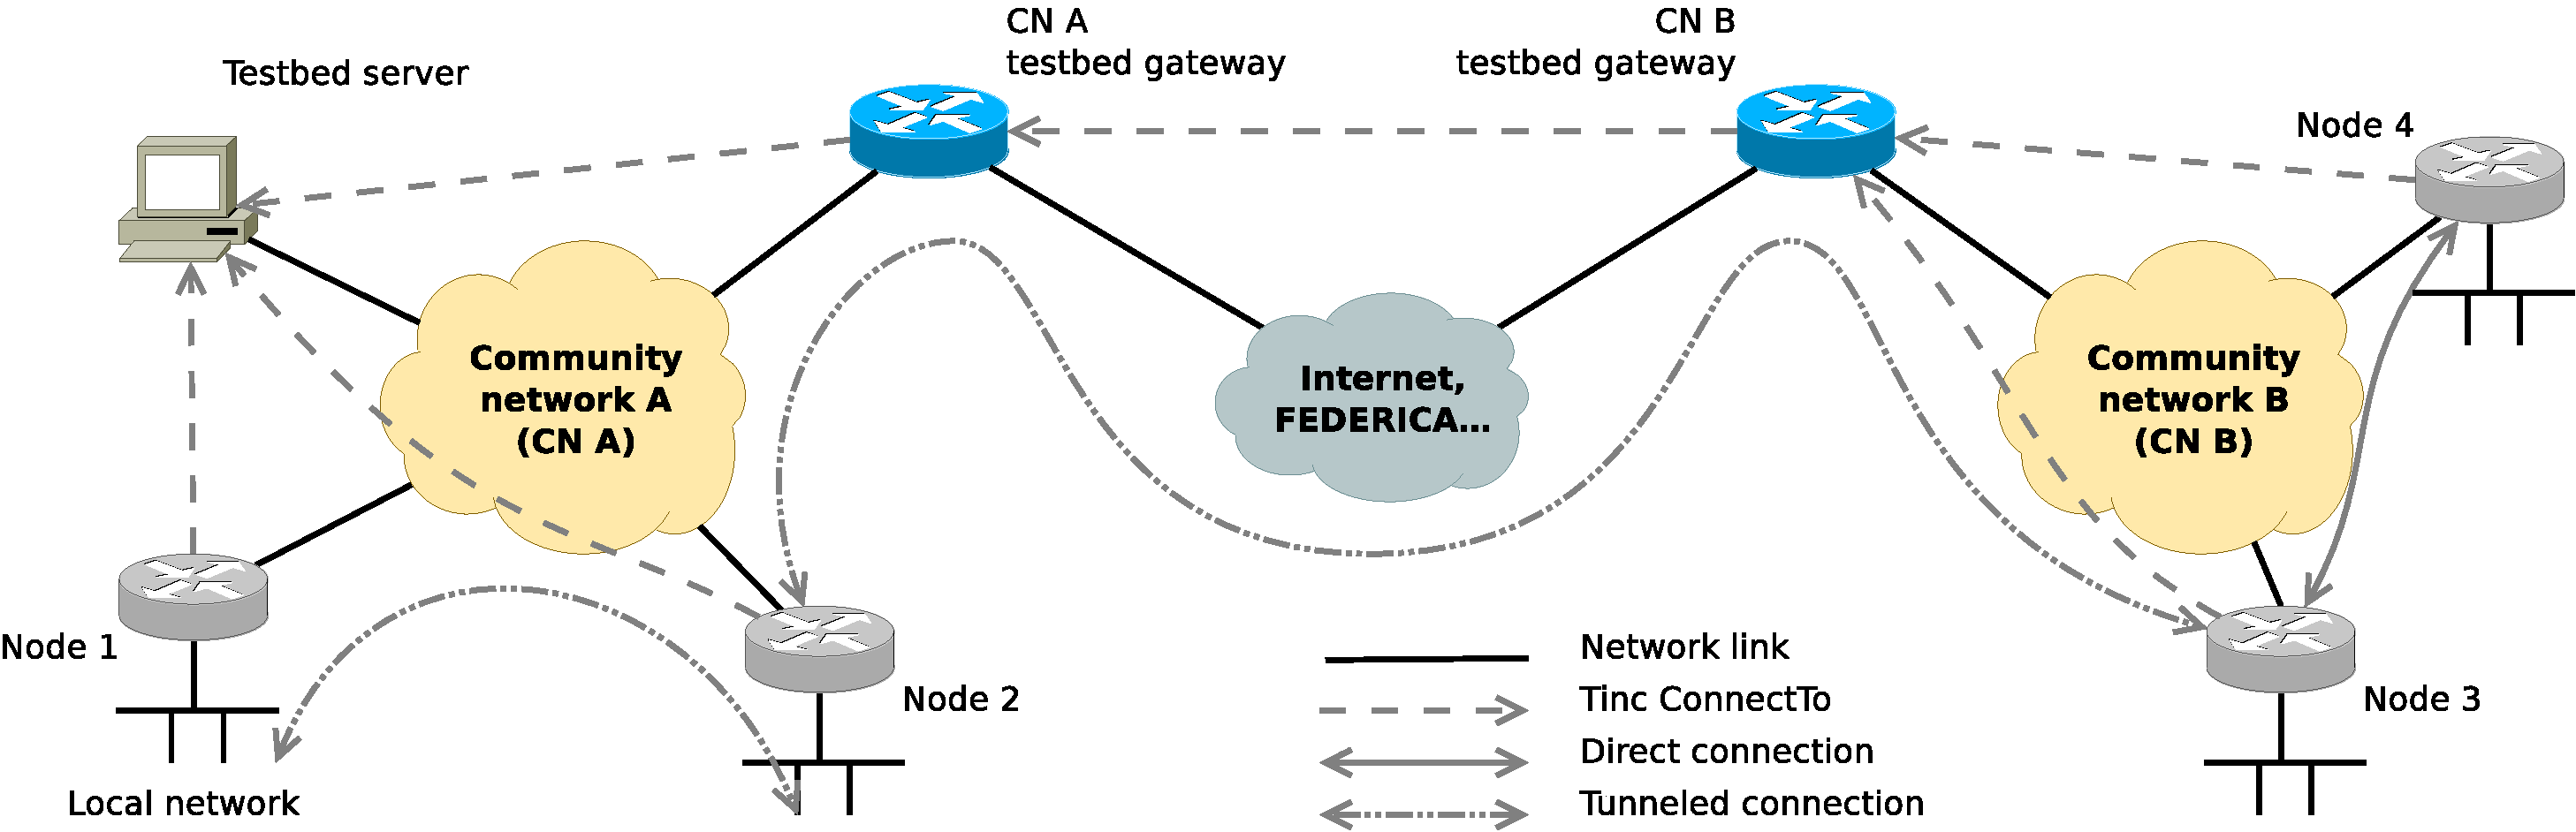
\includegraphics[height=0.20\textheight]{ipv6-overlay}
\caption{The IPv6 overlay spanning two community networks.}
\label{fig:ipv6-overlay}
\end{figure*}

% openwrt, trunk (upcoming attitude adjustment release) 
% management functions, lua-based API, user interfaces based on 
% ssh, openwrt/debian linux environment
% supporting:
% Plans for CONFINED release: fix remaining privacy / security protection


% XXXX begin: Axel
% 3.2 current state
% - implementation (target CONFINED)



At the time of writing this document (end of May 2012) we are just
finishing our first release of the CoNFINE Node System (CNS) for RDs
\cite{a-hack}. The main objective of this first version is to provide
a proof-of concept for selected technologies and be able to gather
experience from the execution of first experiments on real
deployments.

CNS is built on top of the upcoming ``Attitude Adjustment'' release
from OpenWrt \cite{attitudeAdjustment}. The decision to base our work
on the current developer branch (trunk) of OpenWrt was a trade off
between the requirement to provide up-to-date implementations for
quite a number of relatively new Linux networking and virtualization
technologies and the lack of maturity that comes with development
branches. 

The current implementation provides role-specific APIs and user
interfaces for node owners, testbed management, and researchers.

By default, the task of integrating a new testbed RD into an existing
CN is under the control of the node owner.  After the initial flashing
of the RD with our firmware image (implementing the CONFINE node
system for a pre-selection of supported X86 hardware like Alix or
Commell), a node system must be customized for its specific deployment.
Therefore, a small set of testbed- and node-specific attributes
(node ID, public keys...) must be exchanged between the node owner
and the testbed operators via a central web portal and used to
complete the configuration template of the RD.  The
node-management functions \texttt{confine\_node\_enable/disable} can be used at
any time to cleanly activate or deactivate the participation of the RD
in the testbed.

% XXXX uci: http://wiki.openwrt.org/doc/uci "Unified Configuration Interface"

The abstract concept of a sliver is realized via virtualization.  To
provide researchers with a common experimentation environment we
decided to use Linux Container (LXC \cite{lxc}) as a very light-weight
virtualizatinon solution. This allows us to grant researchers root
access to an OpenWrt or Debian guest system (the sliver), but running
completely under control of the CONFINE RD host system. LXC user-space
tools have been ported to OpenWrt as a new package and are used by
the CNS to control the LXC container internally. This sliver
environment given by the container OS can be further extended by the
researcher with additional tools, data, and init scripts to
automatically execute the processes that define experiments.
Interactive access to slivers is provided at any time via SSH and the
Community-Lab management network (\emph{tinc} IPv6 overlay, see next point).

The role of the testbed operators is to manage the deployment and life
cycle of experiments (via the concepts of slices and slivers). The
following set of functions were implemented as Bash scripts for remote
invocation (via SSH and the CONFING management network) from a central
server of the testbed.
\begin{itemize}
\item \texttt{confine\_sliver\_allocate} is used to allocate the resources
  (like local namespaces, IP addresses, storage) on a RD that are
  necessary to execute an experiment. The function requires a sliver
  description in UCI syntax specifying the required interfaces,
  addresses and OS type. On success, it returns precise information
  about the allocated sliver attributes. The attributes of all slivers
  of a slice must be collected by the server for later summarization
  and provisioning as slice attributes during the deployment of each
  sliver. Thereby, each sliver has access to the sliver attributes (e.g. IP
  addresses) of all other slivers in its slice before it is started.
\item \texttt{confine\_sliver\_deploy} is used to setup the sliver environment
  in a RD. Therefore a linux container and root file system is created
  and customized according to RD, slice, and sliver specific
  attributes.  The function requires the slice attributes in UCI
  syntax as input.
\item \texttt{confine\_sliver\_start}, \texttt{confine\_sliver\_stop},
  \texttt{confine\_sliver\_remove} can be used to start, stop, and remove the
  LXC container related to a given sliver (in the RD where the command
  is invoked). The last function does also release all allocated
  resources reserved for that sliver.

\end{itemize}


% XXXX end: Axel



\subsubsection{The IPv6 overlay}

Creating testbeds that span several community networks (CNs) is drastically
hampered by their lack of widespread IPv6 support.  They normally use private
IPv4 addressing that
%(in spite of initiatives like Free Networks \cite{free-networks})
can not be trusted to be compatible across CNs.  Also,
the diversity of CN devices using IPv4 mean that research devices may sit
behind NAT boxes or firewalls further limiting their reachability.  IPv4
address scarcity also keeps the testbed from using a clean and uniform
address scheme for their elements.

% XXXX free-networks: http://freenetworks.org/ "Free Networks association"

IPv6 migration solutions like 6to4 \cite{6to4}, 6in4 \cite{6in4},
or Teredo \cite{teredo} either have problems with protocol 41
handling in NAT boxes or firewalls, or they use host IPv4-based addresses which can
also clash between CNs.  Together with most VPN solutions they get complicated to
setup in a mesh-like cloud, or use centralized architectures which alter the
resulting topology and can turn the VPN server into a bottleneck --e.g. OpenSSH.

% XXXX 6to4: http://www.ietf.org/rfc/rfc3056.txt "Connection of IPv6 Domains via IPv4 Clouds" IETF RFC 3056
% XXXX 6in4: http://www.ietf.org/rfc/rfc4213.txt "Basic Transition Mechanisms for IPv6 Hosts and Routers" IETF RFC 4213
% XXXX isatap: http://www.isatap.org/ "Intra-Site Automatic Tunnel Addressing Protocol (ISATAP)"
% XXXX teredo: http://www.ietf.org/rfc/rfc4380.txt "Teredo: Tunneling IPv6 over UDP through Network Address Translations (NATs)" IETF RFC 4380

\begin{figure*}[!t]
 \centering
 \subfloat[][Community network deployment]{%
      \label{fig:community_network_simple}%
      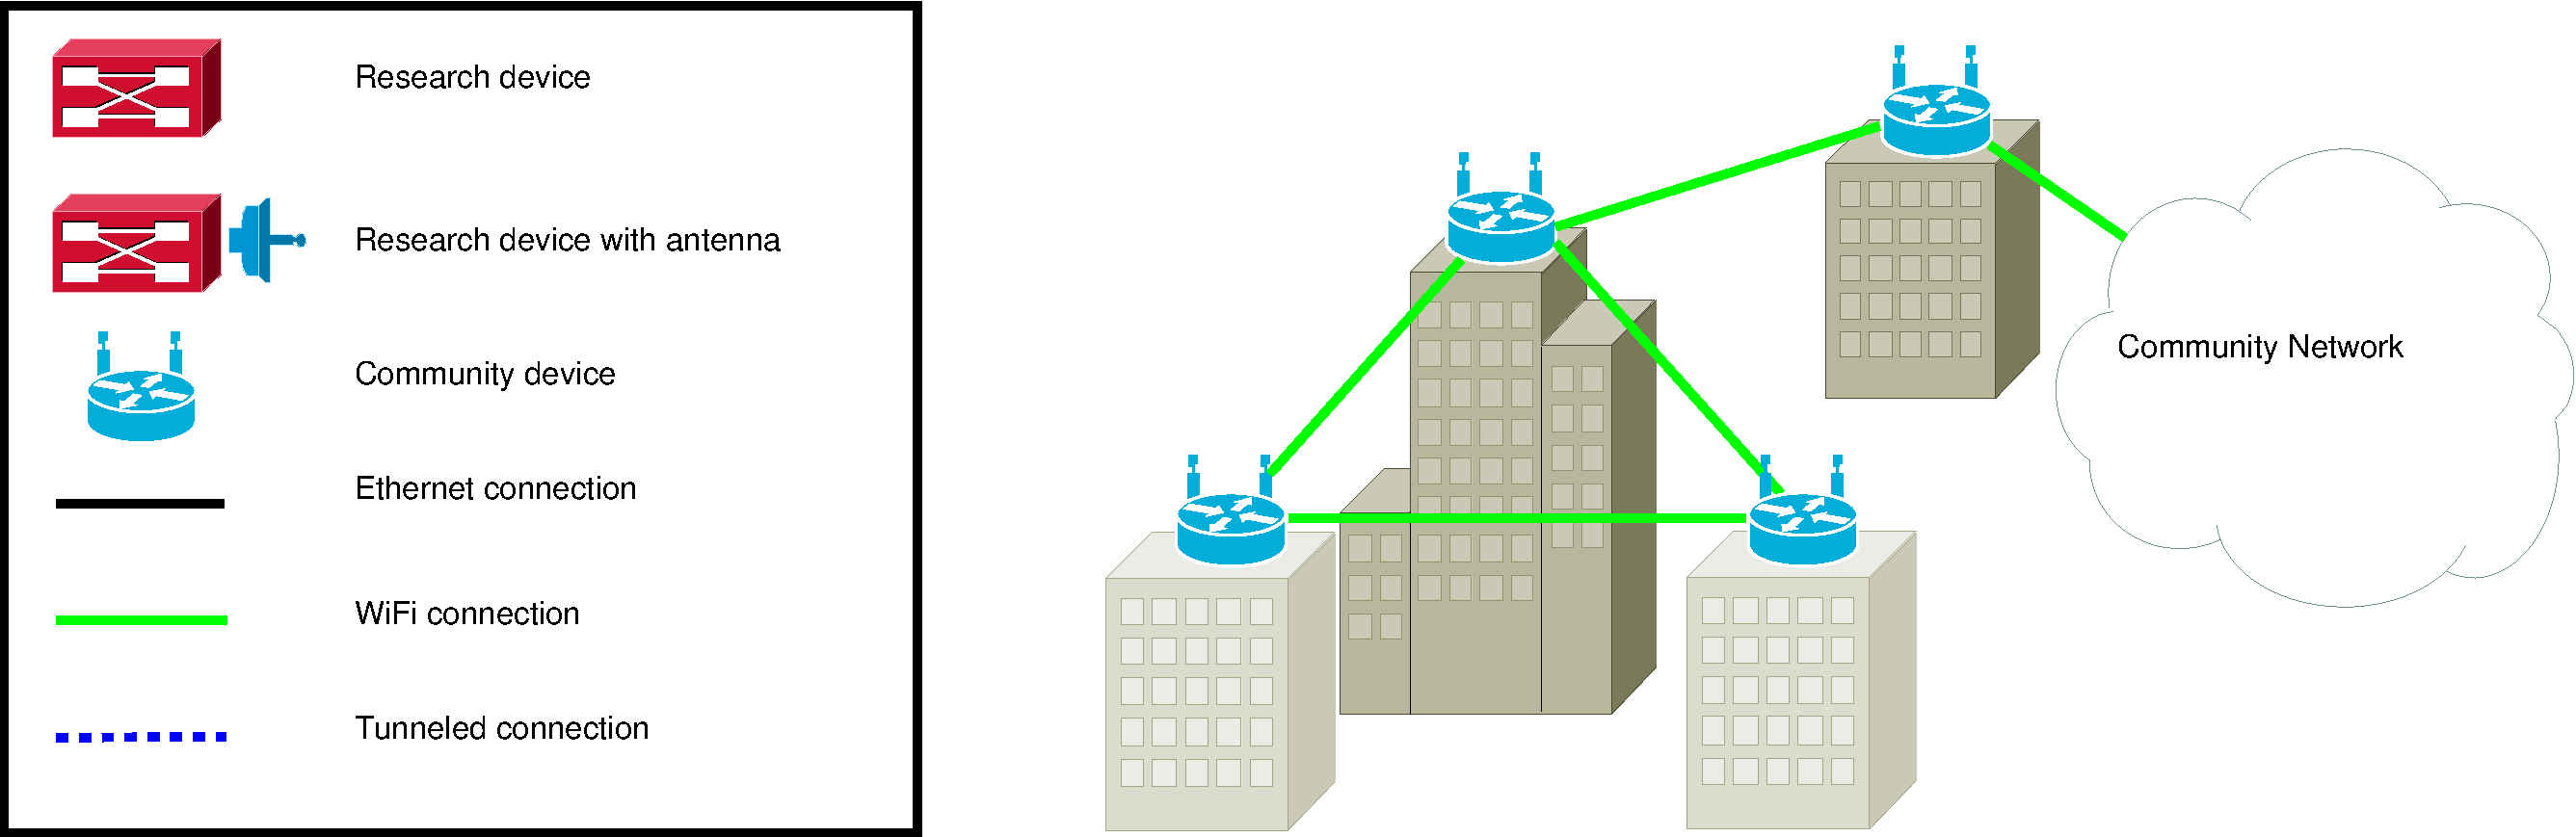
\includegraphics[height=0.20\textheight]{community_network_integration-1}}\\
 \subfloat[][Research devices connected to existing community devices (left) and a complete Community-Lab cloud with community and research devices (right)]{%
      \label{fig:community_network_integration}%
      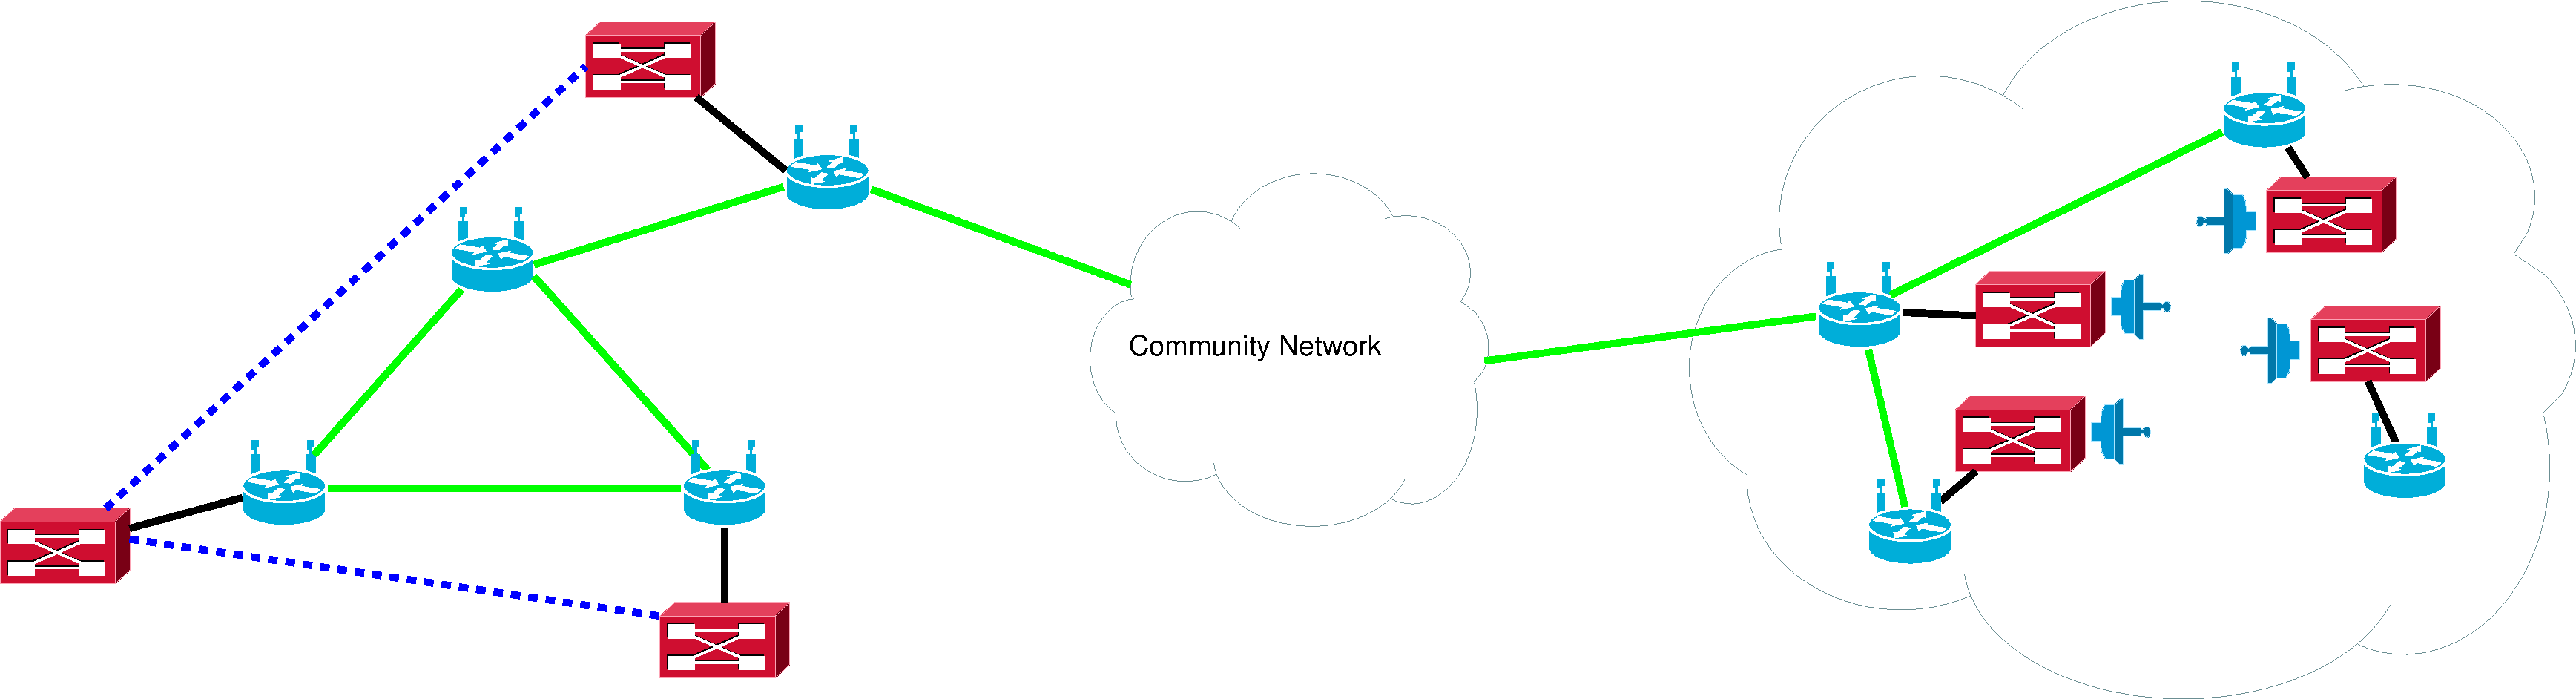
\includegraphics[height=0.20\textheight]{community_network_integration-2}}
 \caption{Community-Lab integration with existing community networks.}
\end{figure*}

A CONFINE testbed works around these problems by creating an \textbf{IPv6
  overlay} based on the \emph{tinc} \cite{tinc} VPN software.  \emph{Tinc}
allows setting up a mesh network where data is exchanged directly between
endpoints with the VPN software taking care of routing traffic and propagating
endpoint information, thus needing minimal configuration.

As shown in figure \ref{fig:ipv6-overlay}, a \emph{tinc} daemon in a testbed
node only connects to the testbed server or a CN testbed gateway.  Gateways
connect between themselves through another network like the Internet.
Together they form a single routed IPv6 network where individual hosts
(servers, gateways and clients) and subnetworks (node devices and slivers)
become available to one another.

Since the overlay makes all elements in the testbed easily reachable through
predictable IPv6 addresses with automatic encryption and authentication
between endpoints, the IPv6 overlay is used as a \textbf{management network}
while CNs gain widespread IPv6 support.

% XXXX tinc: http://www.tinc-vpn.org/ "tinc"

%\subsection{Next steps}
%3.3 next steps
%- 2n year implementation (between CONFINED and envisioned)




\subsection{Community-Lab integration in existing community networks}

What makes the Community-Lab testbed different from existing ones is the integration
with actual community networks (CNs). The nodes belonging to the testbed are deployed among the 
community network to be able to perform experiments in a real enviroment with real users. However 
these networks are indeed production networks, so the experiments must have some limitations or provide some
degree of protection to community network owners. For instance, nodes placed in the core of the network
cannot, as a general rule, execute link layer experiments because it can easily disrupt the correct
operation of the production environment.




% \begin{figure*}[!t]
% 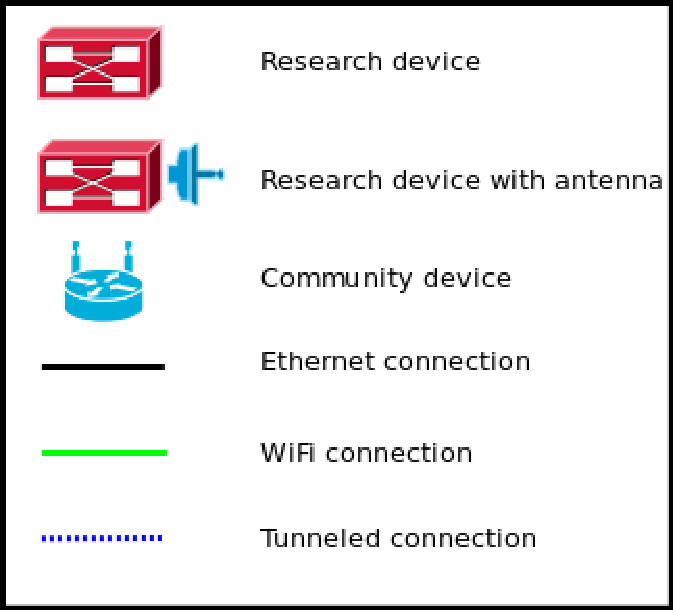
\includegraphics[height=0.12\textheight]{community_network_lengend}
% \centering
% \caption{Legend}
% \label{fig:community_network_lengend}
% \end{figure*}

Community networks have multiple owners, i.e. they conform a \textit{distributed property}, 
which means that each user is the owner of his own device. In a city, where people live in 
buildings, the users normally share a single device placed on the roof -- a good practice though
not always possible.

A typical community network deployment looks like figure \ref{fig:community_network_simple}.
The green lines represent WiFi links. Most of these networks are using this technology because 
it is cheap, easy to use and can be easily obtained. However it might be any other kind of technology 
such as WiMax, Ethernet or Optical Fiber depending on the owner's needs.

% \begin{figure*}[!t]
% \centering
% 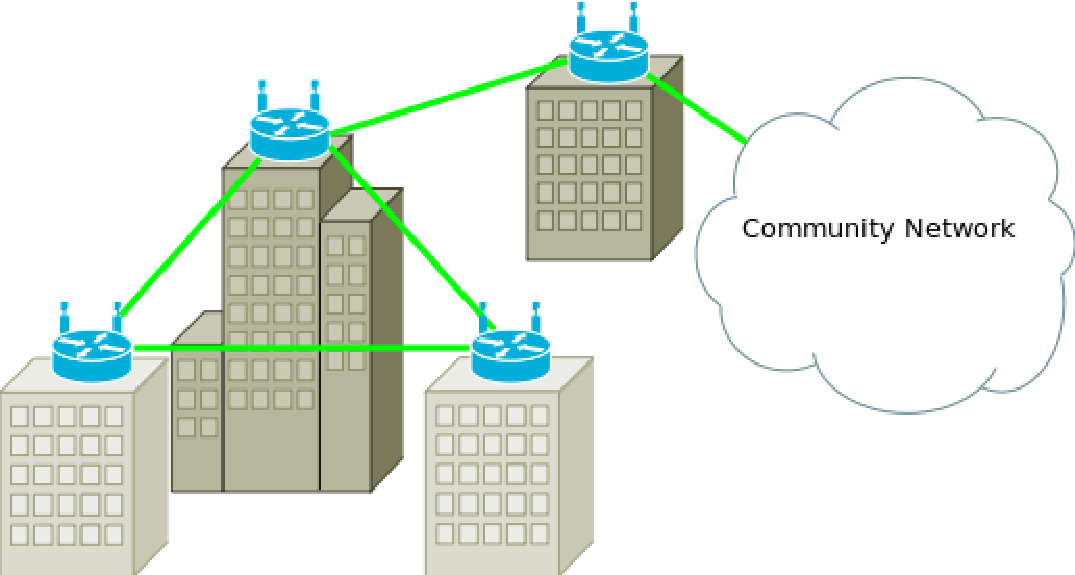
\includegraphics[height=0.20\textheight]{community_network_simple}
% \caption{Community network connection example.}
% \label{fig:community_network_simple}
% \end{figure*}

The integration of the Community-Lab devices inside existing CN requires the collaboration of at least
one part of the community. To make it possible, the CONFINE project provides additional resources in exchange
of covering some of the costs like new links or new nodes. We envision three different levels of integration.

\subsubsection{Single research devices connected to existing nodes}
\label{sec:single-research-devices}

As shown in figure \ref{fig:community_network_integration} (left), a research device (RD) without antennas is 
adopted by a community user not necessary related with the project.
The RD will be connected to the community device (or CD, which is owned by the person who adopts it) through an Ethernet connection. 
The research device will obtain a valid community network IP -- depending on the availability of a DHCP server on the community device --
and it will be reachable from the rest of the network and from the Community-Lab server.
Experiments between research devices can be performed, however restricted to application layer experiments because of the 
lack of direct access to the physical layer. If the owner allows it, a WiFi antenna might be 
added to the research device to allow researchers to obtain valuable link layer information, which could
be usefull to perform long term studies on the real usage of such links.

In this case the CONFINE project only needs to install a single device (the RD) because it uses a existing
CD owned by the user. 

% \begin{figure*}[!t]
% \centering
% 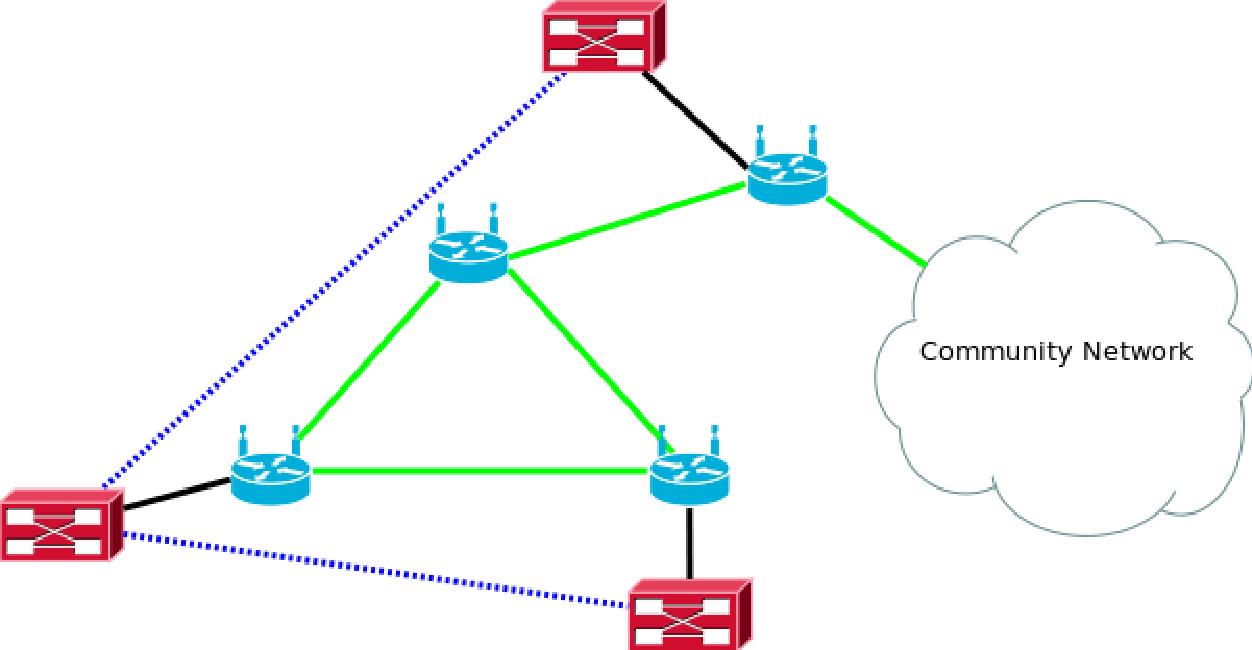
\includegraphics[height=0.20\textheight]{community_network_with_rd}
% \caption{Single research devices connected to an existing node}
% \label{fig:community_network_with_rd}
% \end{figure*}

\subsubsection{Nodes to extend the current network}

One of the explicit objectives of the CONFINE project is to support the growth and usage of this 
\textit{distributed property} network model. In some cases where the community network needs one or 
several extra links to improve performance or availability, the project will
contribute to provide extra resources. These resources will be placed in some community 
member's location, and so the adoption of a research device (following the integration model 
described before) will be a requirement. In this case the CONFINE project will add a new CD and the common RD.

\subsubsection{Multiple nodes (cloud) deployed in a specific scenario}

In some specific scenarios controlled by a CONFINE partner -- i.e. university campus -- an entire cloud may be 
deployed. As shown in figure \ref{fig:community_network_integration} (right), it implies the installation of several 
nodes. The CD must be a node compatible with the existing CN to be able to connect to it. 
The RD may contain one or several WiFi antennas and radio devices depending on the characteristics of the experiments to perform. 
Having several radio devices will allow researchers to execute any kind of link layer experiments given that
the access to the physical layer will be exclusive.

If the set of links (between the nodes) are interesting for the community, the users may make use of them.
Moreover, they must be aware that such a cloud is an experimental network and its availability and stability cannot
be guaranteed. However, this bilateral open access between community network users and researchers can provide
highly valuable information to evaluate new protocols and services.

In this case the CONFINE project will add the new CD, the common RD and any other hardware needed (like wires,
metallic mast, electricity box, etc.).



% \begin{figure*}[!t]
% \centering
% 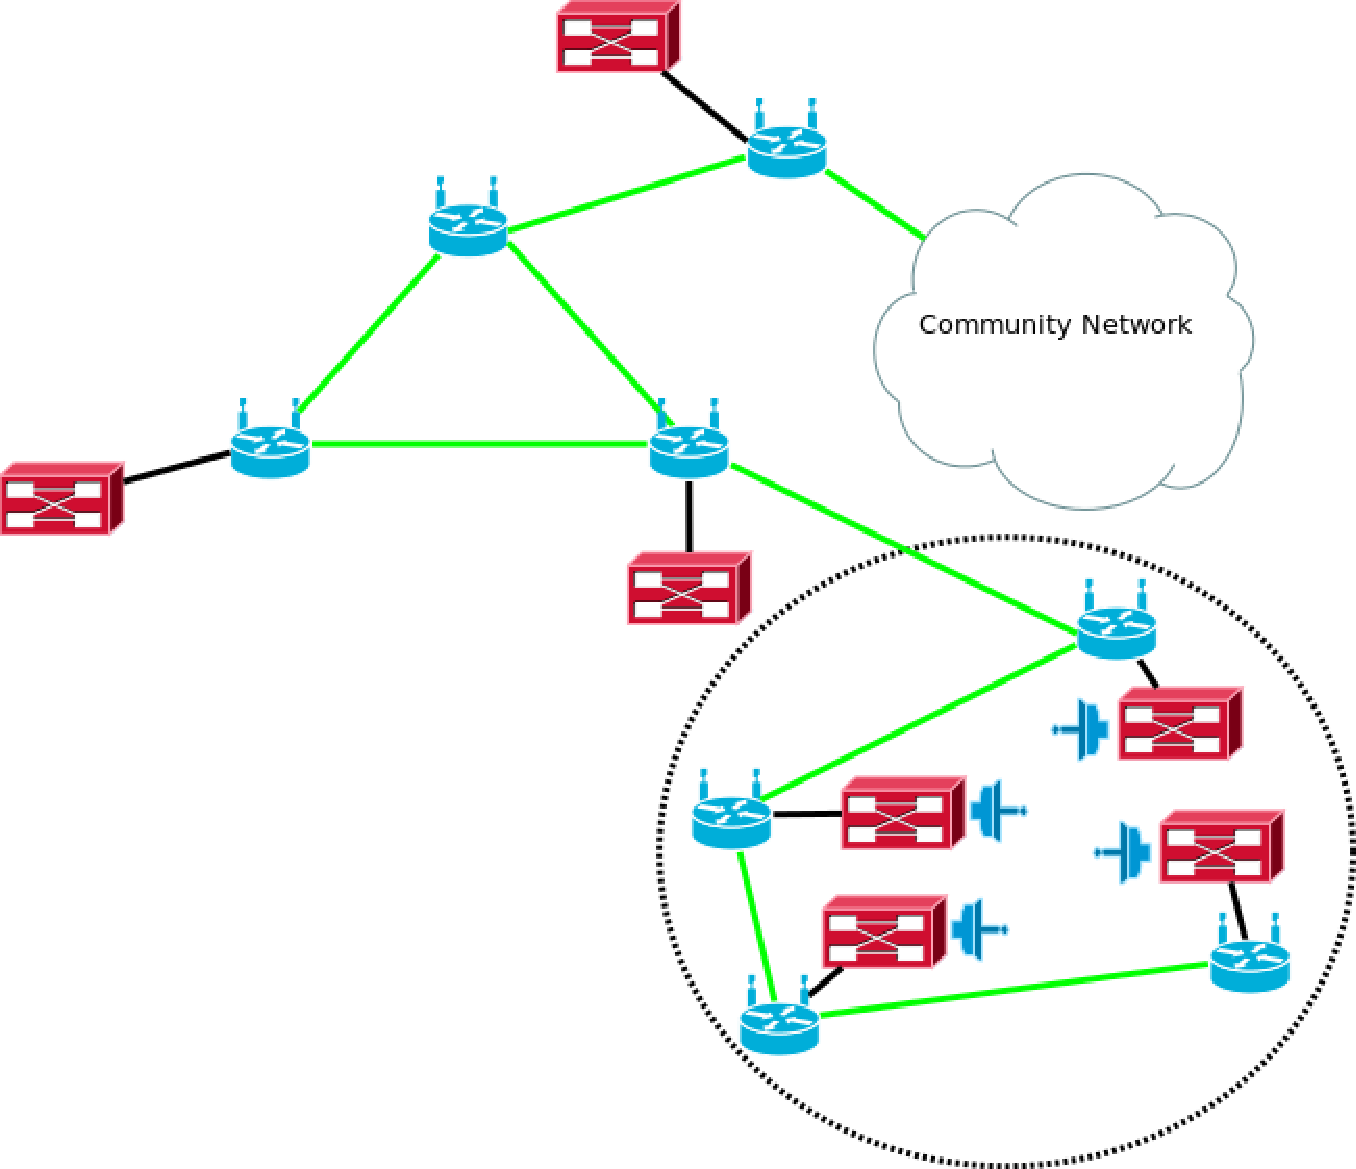
\includegraphics[height=0.25\textheight]{community_network_with_cloud_rd}
% \caption{Multiple nodes of a CONFINE cloud}
% \label{fig:community_network_with_cloud_rd}
% \end{figure*}


%\begin{figure}[!t]
%\centering
%\includegraphics[width=2.5in]{myfigure}
% where an .eps filename suffix will be assumed under latex, 
% and a .pdf suffix will be assumed for pdflatex; or what has been declared
% via \DeclareGraphicsExtensions.
%\caption{Simulation Results}
%\label{fig_sim}
%\end{figure}


%\begin{figure*}[!t]
%\centerline{\subfloat[Case I]\includegraphics[width=2.5in]{subfigcase1}%
%\label{fig_first_case}}
%\hfil
%\subfloat[Case II]{\includegraphics[width=2.5in]{subfigcase2}%
%\label{fig_second_case}}}
%\caption{Simulation results}
%\label{fig_sim}
%\end{figure*}

\subsection{Discussion}

There are three major characteristics which make the Community-Lab
testbed of the CONFINE project unique compared to the deployments presented in section \ref{sec:related-work}: i) the 
larger scale of the testbed with an expected size of thousands of nodes by the end of the project compared to the few tens
of nodes of current deployments; ii) the integration within already existing production community networks which provides
a more realistic scenario for experimentation oposed to controlled lab environments; iii) the support for long term studies
of new network protocols and parallel experimental services which share the same wireless infrastructure -- both from the testbed and from the participating wireless community networks -- by means of
node and network virtualization oposed to other testbeds which provide dedicated nodes to testbed users.
Of course, the development of current deployments presented in this section can and should provide a solid foundation for building
this unique infrastructure.

\section{Conclusion}

Community networks are an emerging field to provide citizens with connectivity in a sustainable and
distributed manner in which the owners of the networks are the users themselves. Research on this field
is necessary to support CNs growth and scope, and improve their operation and quality. However, a few initiatives
have arised to provide researchers with a platform to conduct such novel experimentation which must
push forward this new networking model. The CONFINE project aims to fill this gap by deploying Community-Lab,
a testbed for community networks inside existing community networks. 

Throughout this paper, we have presented the motivation, requirements and challenges that pose the deployment
of such testbed. We have described our envisioned architecture and specified the decisions made during
the design process taking into account the challenges and peculiarities of CNs. Our next step is to make this
architecture a reality for researchers to experiment with novel protocols and services which should
provide community network owners, operators and citizens overall a better experience.

\section*{Acknowledgment}

This work is supported by the European Community Framework Programme 7
within the Future Internet Research and Experimentation Initiative
(FIRE), Community Networks Testbed for the Future Internet (CONFINE),
contract FP7-288535.





% trigger a \newpage just before the given reference
% number - used to balance the columns on the last page
% adjust value as needed - may need to be readjusted if
% the document is modified later
%\IEEEtriggeratref{8}
% The "triggered" command can be changed if desired:
%\IEEEtriggercmd{\enlargethispage{-5in}}

\bibliographystyle{IEEEtran}
\bibliography{confine-cnbub}

\end{document}



%%  LocalWords:  testbed testbeds CN CNs GSM SMS anonymization reachability
%%  LocalWords:  RD's vSwitch
